                               %----------------------------------%
                               % Manhattan College Math Dept      %
                               % Student Homework Template v1     %
                               %    R. Goldstone, 1/1/2011        %
 	               % Edited by T. McGrail, 2/11/2011  %
 	               % Edited by R. McGovern, 8/16/2011 %
 	               % Edited by J. Kirtland, 1/20/2015 %
                               %----------------------------------%
% PREAMBLE ============================================================================

\documentclass[12pt]{article}
\usepackage[utf8]{inputenc}    % set input encoding so bullets are printed
\usepackage{amssymb,amsmath,amsthm}
\usepackage{listings}
\usepackage[usenames,dvipsnames]{color}
\usepackage{matlab-prettifier}
\usepackage{graphicx}

 
% FILL-IN, THEN GO TO DOCUMENT MAIN BODY **********************************************
% TEXWORKS: USE CTRL-TAB TO JUMP FROM INPUT FIELD TO INPUT FIELD
\newcommand{\myname}{Amy Pitts} % Enter name
\newcommand{\duedate}{May 15, 2019} % Enter date, e.g., April 1
\newcommand{\courseno}{440L}      % Enter course number (just the number)
\newcommand{\coursename}{Machine Learning}    % Enter course name
\newcommand{\instructorname}{Instructor: Dr. Pablo Rivas} % Enter instructor name
\newcommand{\assignumber}{}   % Enter assignment number#.
\newcommand{\exerciselist}{Questions 1,2}      % Enter problem references.  Give a complete list, in order, of all of the problems that you will do on this assignment.  Use the format 2.20 to designate problem  # 20 from chapter 2 of the text.
\newcommand{\spacingfactor}{2}
% END FILL-IN *************************************************************************

% DOCUMENT STRUCTURES -----------------------------------------------------------------

% PAGES
\usepackage[paper=letterpaper, margin=1in, headsep=20pt]{geometry}
  
\newcommand{\firstpageinfo}  
    {\textsf{\large\myname}    \hfill     Data \courseno{:}\,\coursename \\
    Final Exam \assignumber \hfill  Due:  \duedate \\
  \instructorname}
% END PAGES

% HEADERS AND FOOTERS
\usepackage{fancyhdr}
\pagestyle{fancy}              % Headers and footers for page 2 and beyond
  \lhead{\textit{\myname}}
  \chead{\textit{Data \courseno}}
  \rhead{\textit{\textit{Final Exam \assignumber}}}
  \cfoot{\textit{\thepage}}
  \renewcommand{\headrulewidth}{0.4pt}
% END HEADERS AND FOOTERS

% TEXT SPACING
\usepackage{setspace}   %Allows for Doublespacing
\usepackage{ifthen}   %Used to create a response environment
% END TEXT SPACING

% PROBLEM AND RESPONSE ENVIRONMENTS
 \newcommand\myqed{}                 % creates command for tombstone at end of proof
\newcommand{\printmyqed}[1][]       % decides whether to print tombstone or not
  {%
  \ifthenelse{\equal{#1}{Proof}}
  {\renewcommand{\myqed}{\qed}}
  {\renewcommand{\myqed}{}}
  }

\newenvironment{exercise}[1][]{%
  \bigskip                          % Space before problem statement
  \noindent \textsf{Exercise #1.}\slshape }{}
   
\newenvironment{response}[1][\textit{Solution}]{%
  \printmyqed[#1]
  \begin{spacing}{\spacingfactor}
  \medskip                          % Space before solution
  \noindent \textit{#1.}}{\myqed\end{spacing}\medskip\hrule}
% END PROBLEM AND RESPONSE ENVIRONMENTS

% =====================================================================================

\begin{document}
\thispagestyle{empty}

% TOP MATTER --------------------------------------------------------------------------
\noindent\firstpageinfo
\begin{center} \underline{\textsf{Exercise List}}\\[5pt] \exerciselist \end{center}
\medskip\hrule
% END TOP MATTER ----------------------------------------------------------------------


%----------------------------------------------------------------------------------------
\begin{exercise}[1] % Put problem reference inside the brackets
  \textbf{Support Vector Machines:}
  \begin{enumerate}
    \item[a)] Download the python program final.SVM.sinc.py which implements 
    a 10-fold cross-validation approach to find the best set of 
    hyper-parameters $C$, $\epsilon$ (epsilon), and $\gamma$ (gamma), 
    in an Support Vector Machine for Regression (SVR).
    \item[b)] Download the python program finalGenData.py 
    which generates data points of the “sinc” function 
    contaminated with random noise.
    \item[c)]  Modify the program in 1.(a) to run for 1,000 samples, 
    and then report the best set of hyperparameters found. 
    Go here https://goo.gl/forms/X1maf8zSIjPhoyNA2 and report 
    your results. You can do it as many times as you want, 
    but at least one is required.
    \item[d)] \textbf{Explain} your results. How do you interpret the 
    hyper-parameters? Is there a great penalty?
    Is there room for errors without penalty? Is there a 
    relationship between $C$ and $\epsilon$? Any other
    thoughts?
    \item[e)] \textbf{(Extra credit +10)} Repeat 1.(c)-(d) but for 10,000 samples.
  \end{enumerate}
\end{exercise}
  
  
\begin{response}[Solution]

  %\lstset{language=Python,frame=single}
  %\begin{lstlisting}[language=Python,frame=single]
  %\end{lstlisting}
  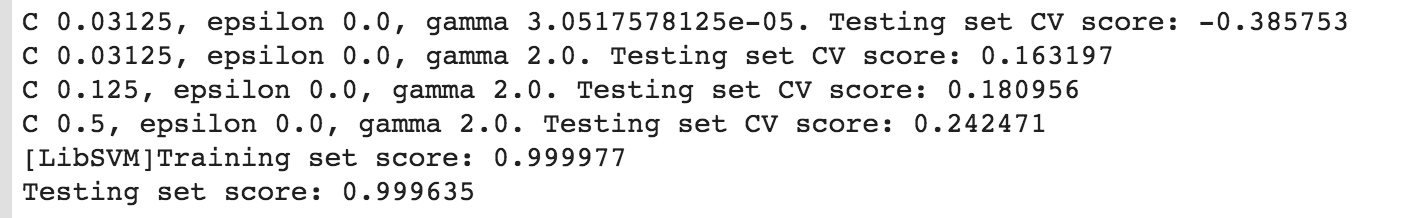
\includegraphics[width=150mm]{final_output_1.png} \\
  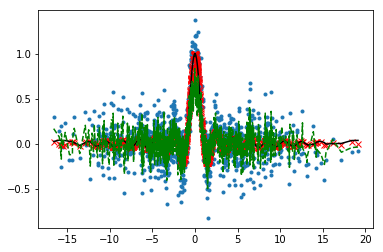
\includegraphics[width=100mm]{hw_1.png} \\
  The best C is 0.5, the best epsilon is 0.0 with the best gamma 
  being 2.  The C is a relatively small value meaning there is 
  not a high error term. The epsilon is very small, meaning that 
  the range of values around $y_i$ is not really a range but 
  rather just the $y_i$ values themselves. The gamma value 
  is a whole number meaning the bell curve is spread out. 

\end{response}
%------------------------------------------------------


\begin{exercise}[2] % Put problem reference inside the brackets
  \textbf{More Support Vector Machines: } For this part you will 
  use the digits dataset. For reading the dataset, you should use 
  the following Python code in a file named finalGetDigits.py:
  \lstset{language=Python,frame=single}
  \begin{lstlisting}[language=Python,frame=single]
import numpy as np
from numpy import genfromtxt

def getDataSet():
  # read digits data & split it into X and y for training and testing
  dataset = genfromtxt('features.csv', delimiter=' ')
  y = dataset[:, 0]
  X = dataset[:, 1:]

  dataset = genfromtxt('features-t.csv', delimiter=' ')
  y_te = dataset[:, 0]
  X_te = dataset[:, 1:]
  return X, y, X_te, y_te
  \end{lstlisting}
  Once saved do the following:
  \begin{enumerate}
    \item[a)]  Download the python program final.SVM.dig.py 
    which implements a 10-fold cross-validation approach 
    to find the best set of hyper-parameters $C$, $\epsilon$ 
    (epsilon), and $\gamma$ (gamma), in an Support
    Vector Machine for Regression (SVR) in the digits dataset.
    \item[b)]  Run the program in 2.(a) and modify it if you 
    need to, to find and report the best set of 
    hyperparameters and the final validation score. 
    Save the plot and interpret it, give your comments
    about it.
    \item[c)] \textbf{Explain} your results. How do you interpret the 
    hyper-parameters? Is there a great penalty?
    Is there room for errors without penalty? Is there a 
    relationship between $C$ and $\epsilon$? Any other
    thoughts?
    \item[d)]  \textbf{(Extra credit +30)} Prepare and share a single 
    Colaboratory for both 1.(c)-(d) and 2.(b)-(c).
    You should use proper headings and comments and 
    explanations. Pro Tip: you may have to
    combine all files into a single program or upload 
    files on demand.
  \end{enumerate}
\end{exercise}
   
\begin{response}[Solution] 
  \textbf{c)} BEST! C 4096.0, epsilon 1.4, gamma 0.0625. Testing set CV score: 0.337201
  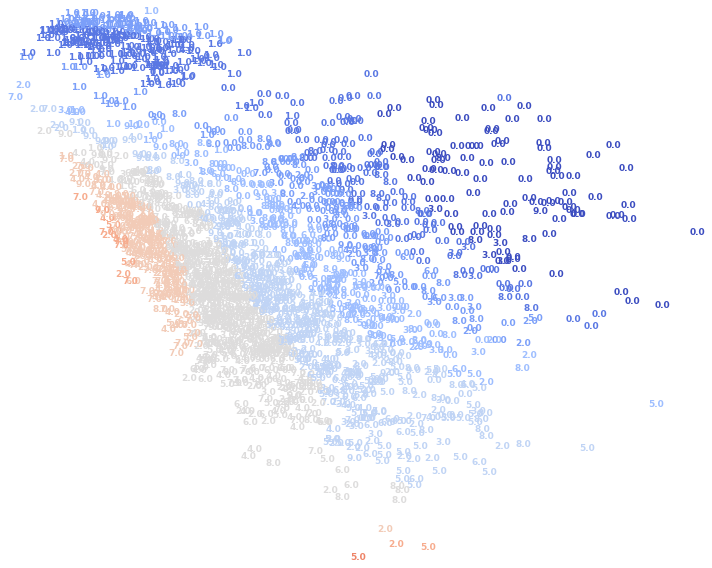
\includegraphics[width=100mm]{final_q_2.png}  \\
  The C value is high which means that there is a high 
  penalty on the error. The epsilon term describes how far away 
  you can be from the $y_i$ values. Since the $y_i$ values 
  represent the numbers that means that the epsilon range is $y_i + 1.4$ 
  and $y_i-1.4$ meaning the range could be + or - a number. The 
  gamma of 0.0625 represent a small bell curve. 

  \textbf{d)} I did put all the work in a google-colab. 
  I shared it with you. My user name is amypitts01. 

  Thank you!


\end{response}




%------------------------------------------------------


\end{document}
%======================================================================================
% END DOCUMENT MAIN BODY ==============================================================
% COPY AND PASTE THIS DOUBLE-SPACE PROBLEM-RESPONSE PAIR AS NEEDED
%======================================================================================



